\chapter{Components \& Containers}

This chapter provides a detailed breakdown of the Coffee Chain ERP system in terms of its \textbf{containers} (modules) and the internal \textbf{components} of each module. Understanding the containers and components is essential for grasping the system architecture and how different parts interact to achieve operational efficiency.

\section*{Definition of a Container}

In the context of Coffee Chain ERP, a \textbf{container} represents a deployable or executable part of the system, such as a web application, microservice, or database, that encapsulates a set of functionality. Containers can be thought of as the high-level building blocks of the system. For example, the Sales Module is a container because it is a standalone web application managing sales transactions, linked to menu and CRM modules.

\section*{Containers of Coffee Chain ERP (C2 Diagram)}

The following containers constitute the Coffee Chain ERP system:

\begin{itemize}
    \item \textbf{Outlet Management:} Web application managing outlet details, managers, and regional assignments.
    \item \textbf{Sales Module:} Web application capturing daily sales, linking products to orders, and generating performance reports.
    \item \textbf{CRM Module:} Web application tracking customer leads, interactions, and supporting targeted marketing.
    \item \textbf{Menu Module:} Web application managing products, categories, and prices, synchronized with Sales.
    \item \textbf{Reporting \& Analytics:} Web application providing dashboards and consolidated performance insights.
\end{itemize}

\begin{figure}[H]
\centering
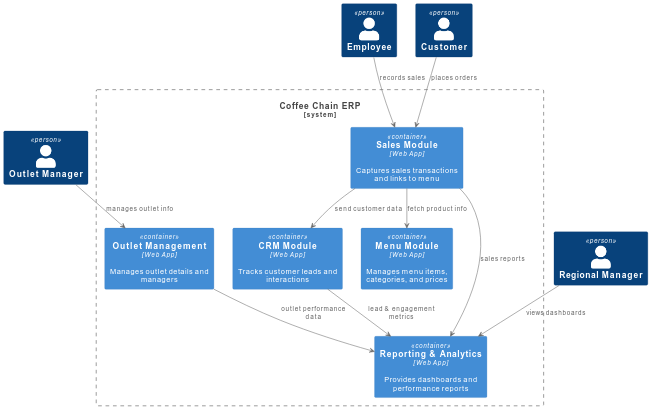
\includegraphics[width=0.9\textwidth,keepaspectratio]{diagrams/C2.png}
\caption{C2-Level Container Diagram of Coffee Chain ERP}
\end{figure}

\subsection*{Insights}

The C2 diagram illustrates how each module (container) interacts with other modules and external actors (employees, managers, customers). This high-level view helps stakeholders understand dependencies, system boundaries, and data flow without needing to inspect individual module internals.

\section*{Components of Each Container (C3 Diagrams)}

Each container is composed of internal components that define its functionality and interactions. These components are depicted in C3-level component diagrams.

\subsection*{Outlet Management Module Components}
\begin{itemize}
    \item Outlet Information Management
    \item Manager Assignment Component
    \item Regional Performance Component
    \item Reporting Component
\end{itemize}

\begin{figure}[H]
\centering
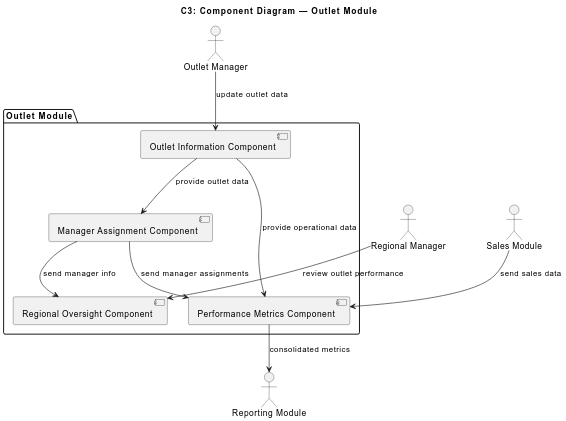
\includegraphics[width=0.9\textwidth,keepaspectratio]{diagrams/C3_outlet.png}
\caption{C3-Level Component Diagram — Outlet Management}
\end{figure}

\subsection*{Sales Module Components}
\begin{itemize}
    \item Transaction Processing Component
    \item Reporting Component
    \item Product Link Component
    \item Payment Processing Component
\end{itemize}

\begin{figure}[H]
\centering
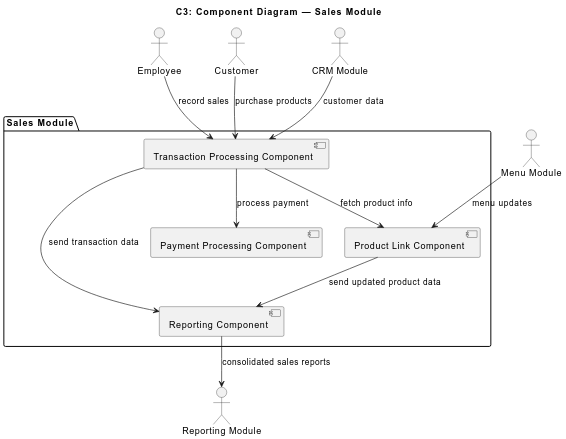
\includegraphics[width=0.9\textwidth,keepaspectratio]{diagrams/C3_sales.png}
\caption{C3-Level Component Diagram — Sales Module}
\end{figure}

\subsection*{CRM Module Components}
\begin{itemize}
    \item Lead Management Component
    \item Customer Interaction Component
    \item Customer Segmentation Component
    \item CRM Reporting Component
\end{itemize}

\begin{figure}[H]
\centering
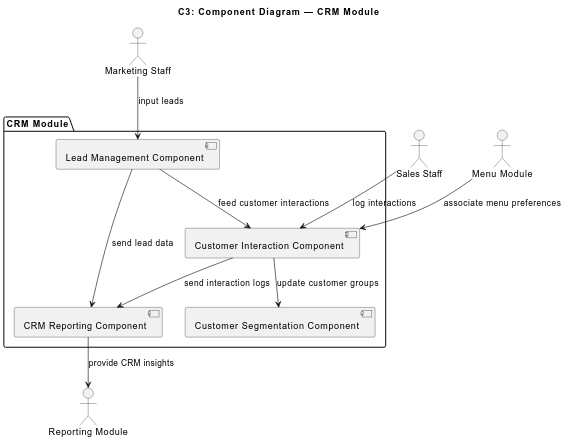
\includegraphics[width=0.9\textwidth,keepaspectratio]{diagrams/C3_crm.png}
\caption{C3-Level Component Diagram — CRM Module}
\end{figure}

\subsection*{Menu Module Components}
\begin{itemize}
    \item Menu Item Management Component
    \item Category Management Component
    \item Pricing Component
    \item Menu-Sales Synchronization Component
\end{itemize}

\begin{figure}[H]
\centering
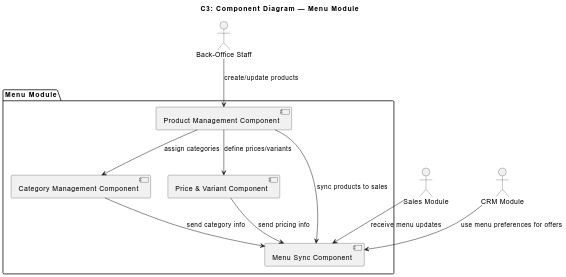
\includegraphics[width=0.9\textwidth,keepaspectratio]{diagrams/C3_menu.png}
\caption{C3-Level Component Diagram — Menu Module}
\end{figure}

\subsection*{Insights}

Analyzing the C3 diagrams reveals the following:

\begin{itemize}
    \item Each module has a clear separation of responsibilities via components.
    \item Internal components communicate with external actors (employees, customers, managers) and other modules to provide seamless operations.
    \item The ERP system’s modular architecture enables future extension, such as adding Loyalty \& Rewards or Inventory Management, without disrupting existing modules.
    \item Real-time synchronization between Menu, Sales, and CRM is critical for accurate reporting and decision-making.
\end{itemize}

